\chapter[Experiment Two: Dual Mappings]{Experiment Two: Dual Mappings}
\label{chap:exp2}
\ifpdf
    \graphicspath{{Chapters/ExperimentTwo/Exp2Figs/PNG/}{Chapters/ExperimentTwo/Exp2Figs/PDF/}{Chapters/ExperimentTwo/Exp2Figs/}}
\else
    \graphicspath{{Chapters/ExperimentTwo/Exp2Figs/EPS/}{Chapters/ExperimentTwo/Exp2Figs/}}
\fi  


A series of experiments was conducted to explore the potentials and limitations of the interactive tag cloud visualisation tool Taggle. Properties of the enhanced tag cloud features utilised in the system were investigated in two experiments using eye-tracking technology to discover if improvements could be made in user performance for visual search tasks. This chapter details the second experiment, where we investigated dual data mappings to font size and colour visual properties. Research questions and goals for the study are presented in \S\ref{sect:experimenttwo}. The methodology of the evaluation is detailed from \S\ref{sect:exp2participants} through \S\ref{sect:exp2hypotheses}. Results from the response times and the eye-gaze data analysis are discussed in \S\ref{sect:exp2results}, with threats to the experiment validity considered in \S\ref{sect:threatsexp2}. Finally, results are summarised and conclusions are presented in \S\ref{sect:exp2summary} and \S\ref{sect:exp2conclusions}.

\section{Single or dual data mappings}\label{sect:experimenttwo}

A special feature of the tag cloud visual encoding in Taggle is that we can use multiple visual features for visualising data variables. Previous research \citep[][]{lohmann09, bateman08, halvey07} shows that different visual features have different effects on user perception when searching for a particular tag. From a software engineering visualisation perspective, this is important as users of our tag cloud tool will need to deal with correlations between data variables mapped to multiple visual features. We wanted to find out what effect mapping dual visual properties had --- if using two visual features such as size and colour together to represent a data field would have an improved user visual search performance than one visual feature. We had the following research question: 

\begin{description}
\item[RQ:]How does mapping a data variable to size or colour compare to mapping a data variable to size and colour together with respect to user performance for search tasks?
\end{description}

We also wanted to find out if a change in layout made a difference to performance. Five tag cloud sets consisting of six tag clouds containing 100 tags each were created within a canvas of $850 \times 650$ pixels (30 tag clouds). Participants saw 24 tag clouds each, plus a trial set of six tag clouds. For details regarding how the canvas size was determined and for tag cloud construction information, see \S\ref{sect:experimentone}.

\section{Participants}\label{sect:exp2participants}
We recruited ten University of Canterbury students to participate in the study (age 18\textendash35, 1 female, with no reported uncorrected vision problems). All had completed, or were completing stage two or three computer science university papers.  Participants received a \$20 gift voucher for participating in the study.

\section{Apparatus}
For details regarding the apparatus used, see \S\ref{sect:apparatusexp1}.

\section{Tag corpora}
Five tag corpora were developed containing 100 data points each, with a categorical variable containing six categories --- refer to \S\ref{sect:tagcorpora} for details.

\section{Procedure}

After completing a demographic questionnaire and signing a consent form, five minutes of training describing tag cloud visualisation was given pre-experiment. 

Participants were shown sets of tag clouds varying data to visual property mappings, and layout, with order counter-balanced using a Latin square design. Each set of tag clouds related to a particular tag corpus, where the target tag was identical for each cloud.  Before each tag cloud, a short text was displayed explaining the scenario and naming a target tag. This text was the same for each cloud set with the scenario adapted to the corresponding tag corpus, and the corresponding visual property hint given. Target tags were selected randomly, with the number of data points within the target category varying between corpus.

The experiment began with a practice tag cloud set containing six tag clouds. Following this, four tag cloud sets containing six tag clouds each (timed trials) were presented (a total of 24 timed trials per participant).

To minimise time and bias, participants performed experiment two and three together, but not experiment one. Overall, participation took 40 to 60 minutes.

\section{Design}
We used a $3\times2$ experimental design for the following within-subject factors and levels:

\begin{itemize}
	\item Mappings \{size, colour, dual\}
	\item Layout \{spiral, typewriter\}
\end{itemize}

The dual level in the mappings factor refers to size and colour visual properties being used together to map the same data variable.

\section{Task}
 
Participants completed a visual search task with a random target belonging to a particular category in a tag cloud containing 100 tags. The target was specifically named and there was only one such target within each tag cloud. The number of tags in the target category was distributed across the repetitions (9, 16, 21, and 48). The scenario for the dataset and specific target was described in the instruction screen before the trial, as shown in Figure~\vref{fig:exp2}. 

\begin{figure}[!htb]
\centering
\begin{subfigure}{.3\textwidth}
  \centering
  \textit{You are about to see names of mines in the US and their operating status.
  		Names with a large font size have the status `Non-producing'. 
  		Find and click on `Dora8' which has status non-producing.}
  \label{fig:instructionsM1Spiral}
\end{subfigure}%
\begin{subfigure}{.7\textwidth}
  \centering
  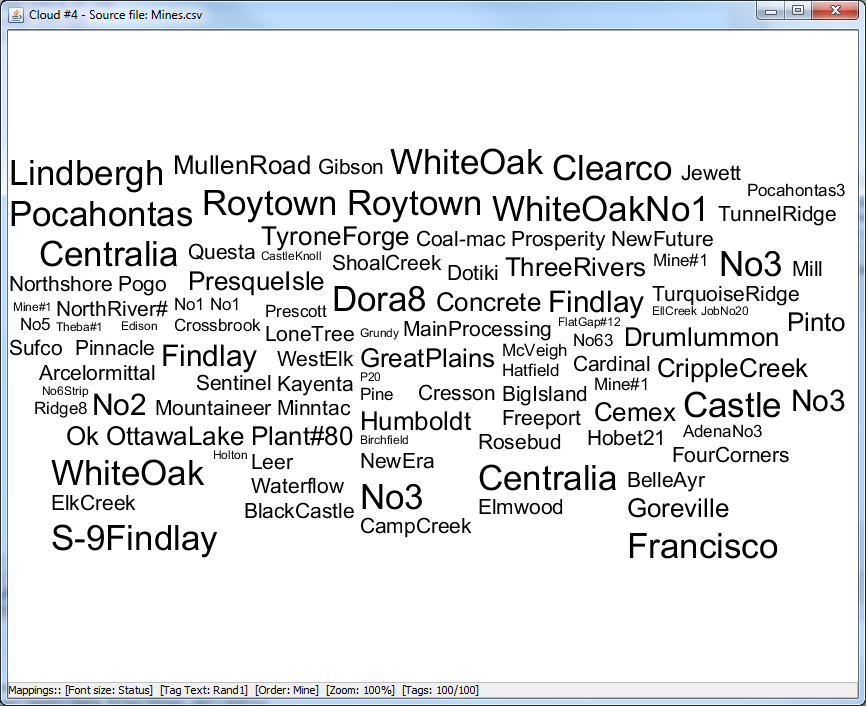
\includegraphics[scale=0.30]{M1Spiral.png}
  \caption{Font size mapping, spiral layout}
  \label{fig:M1Spiral}
\end{subfigure}
\begin{subfigure}{.3\textwidth}
  \centering
   \textit{You are about to see names of mines in the US and their operating status.
 		 Light blue colour names have the status `Non-producing'. 
  		Find and click on `Dora8' which has status non-producing.}
\end{subfigure}%
\begin{subfigure}{.7\textwidth}
  \centering
  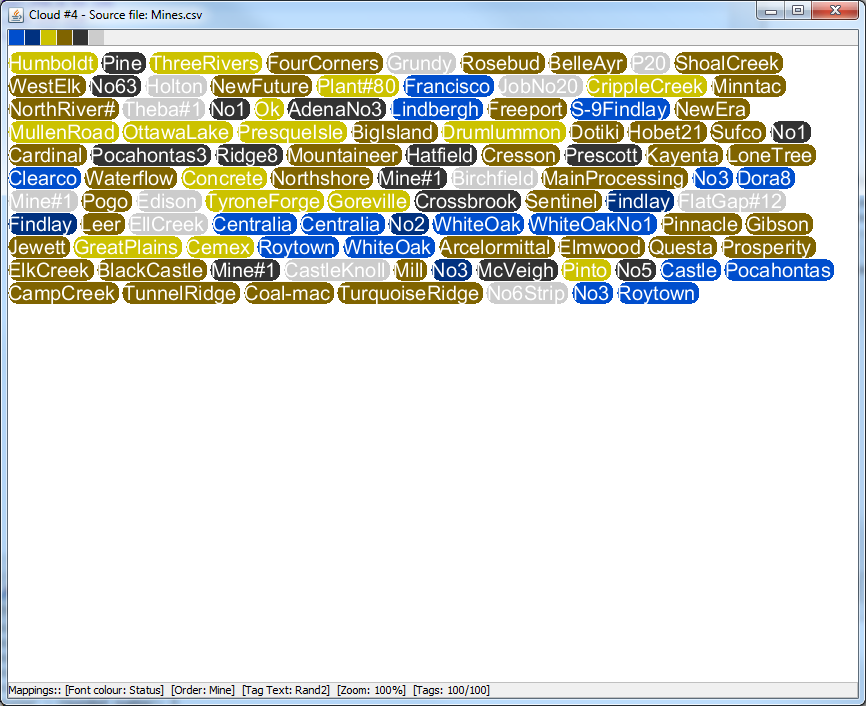
\includegraphics[scale=0.30]{M2Typewriter.png}
  \caption{Tag colour mapping, typewriter layout}
\end{subfigure}
\begin{subfigure}{.3\textwidth}
  \centering
   \textit{You are about to see names of mines in the US and their operating status.
 		 Light blue colour names with a large font size have the status `Non-producing'. 
  		Find and click on `Dora8' which has status non-producing.}
\end{subfigure}%
\begin{subfigure}{.7\textwidth}
  \centering
  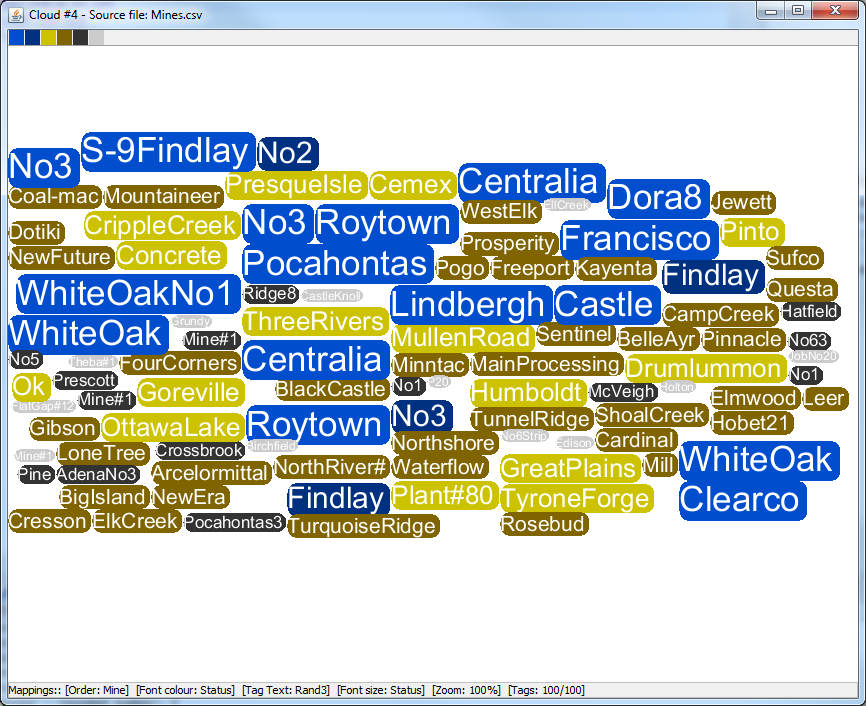
\includegraphics[scale=0.30]{M3Spiral.png}
  \caption{Tag colour + font size mapping, spiral layout}
\end{subfigure}
\caption{\textit{Mapping and layout combinations in experiment two}}
\label{fig:exp2}
\end{figure}

\section{Measurements}

The dependent measure was response time (time to first mouse click on target) -- this is the same as in experiment one, see \S\ref{sect:measurements} for details.

There were no incorrect targets selected in the experiment. In one trial, a participant could not recall the name of the target. This trial was not included in the statistical analysis.

\section{Hypotheses} \label{sect:exp2hypotheses}
 
We defined a hypothesis:

\begin{description}
\item[H1:]\textit{Mapping a data field to tag font size and colour will lead to faster visual search times than mapping a data field to either tag font size or colour separately.}
\end{description}

\section{Results}\label{sect:exp2results}

\subsection{Eye-gaze data analysis} \label{subsect:eyegaze2}
The analysis of the eye-tracking data was performed manually, in an exploratory manner looking for typical patterns in the visual search. As with the eye-gaze data analysis from experiment one, collected data indicates the introduction of a colour hint in tag searches can alter the search strategy, with the eye scan path focusing on tags with the target colour. Refer to \S\ref{subsect:eyegaze} for details describing the search strategies found in tag clouds in experiment one and experiment two.

Visual feature search was found across all three mapping types and all repetitions   (which featured different datasets and a different colour palette where applicable --- see Figure~\vref{fig:featuresearch}). As in experiment one, with datasets containing a larger target category size (such as repetition one --- 48 tags), some participants used chaotic or serial scanning searches to locate the target. 

In repetition two, the target category size was much smaller (21 tags), but gaze analysis showed the tag cloud created for the underlying dataset took up more space proportionally on the canvas than tag clouds from other repetitions (see \S\ref{subsect:responsetime} for further discussion regarding this). With more text to search through (and a longer response time overall), participants appeared to be more likely to switch between search methods. Figure~\vref{fig:chaoticsearch} shows examples from trial repetitions one and two, where participants employed combination searches switching between multiple search strategies.

\begin{figure}[!htb]
\centering
\begin{subfigure}{.5\textwidth}
  \centering
  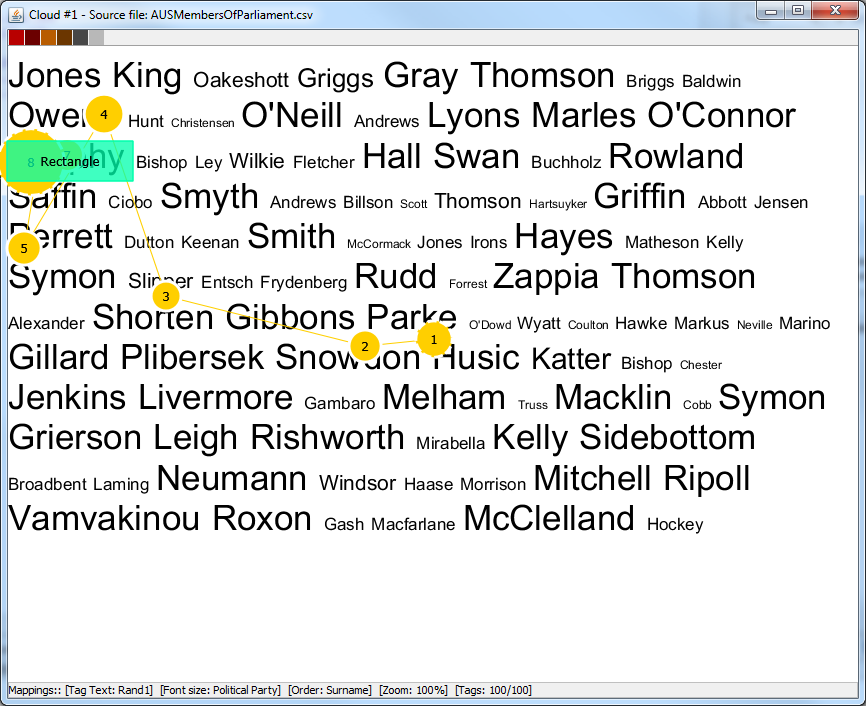
\includegraphics[scale=0.25]{t1featuresearch.png}
  \caption{Repetition one with size mapping}
\end{subfigure}%
\begin{subfigure}{.5\textwidth}
  \centering
  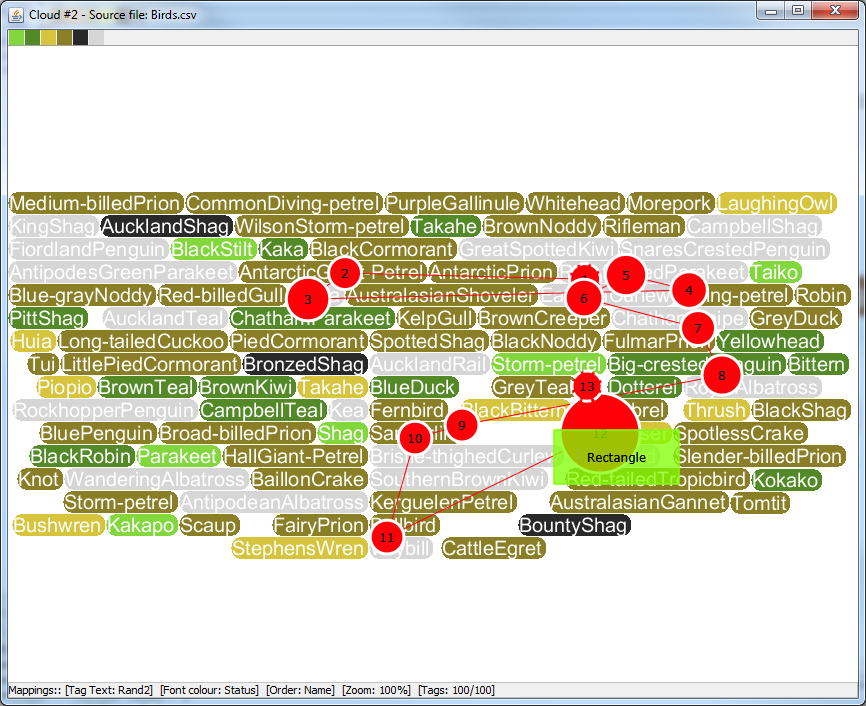
\includegraphics[scale=0.25]{t2featuresearch.png}
  \caption{Repetition two with colour mapping}
\end{subfigure}
\begin{subfigure}{.5\textwidth}
  \centering
  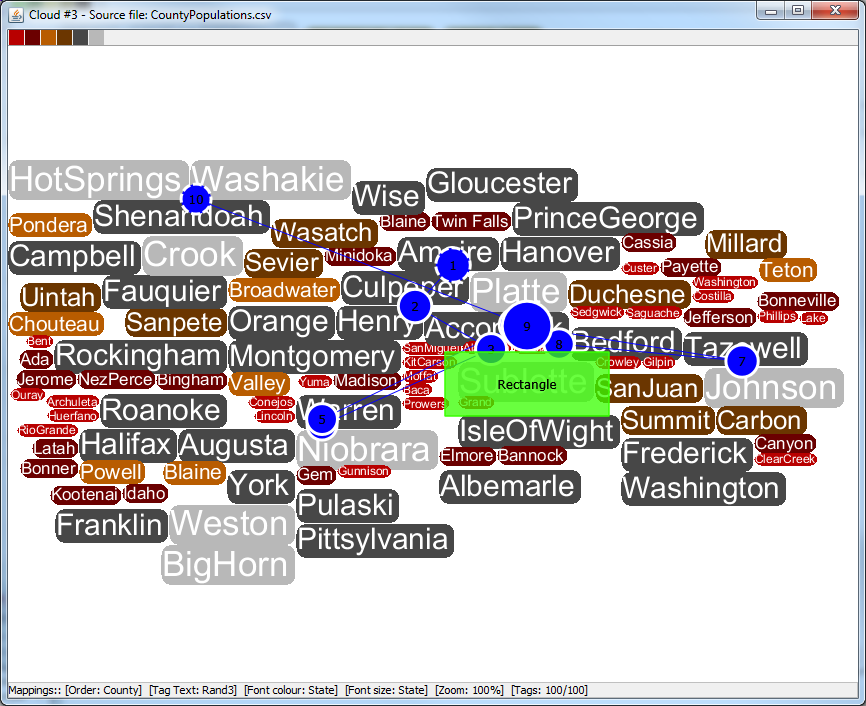
\includegraphics[scale=0.25]{t3featuresearch.png}
  \caption{Repetition three with dual mapping}
\end{subfigure}%
\begin{subfigure}{.5\textwidth}
  \centering
  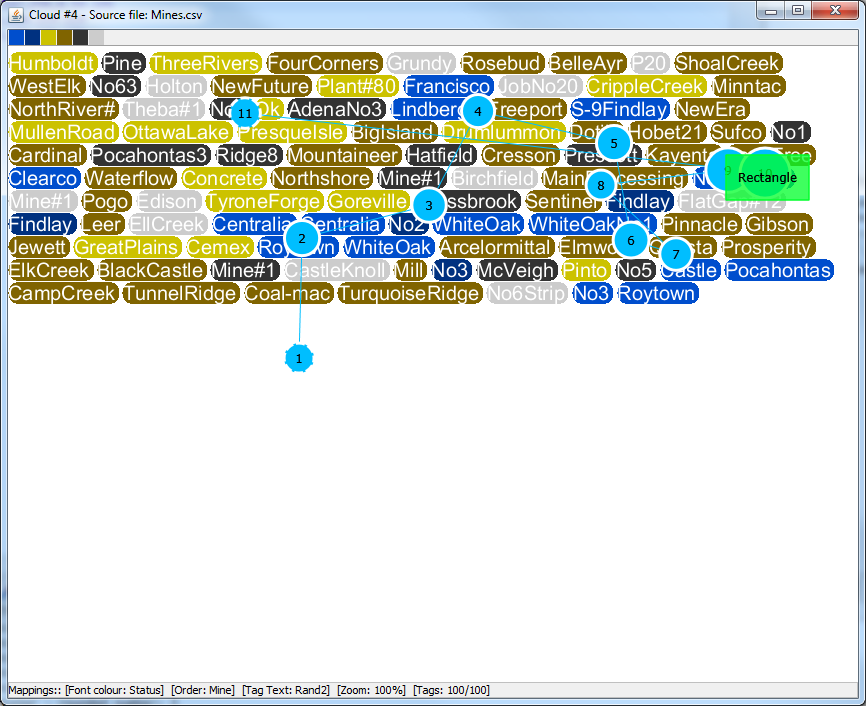
\includegraphics[scale=0.25]{t4featuresearch.png}
  \caption{Repetition four with colour mapping}
\end{subfigure}
\caption{\textit{Visual feature search with fixation clustering around tags with target mapping. Animated visualisations of these examples can be found at \url{http://www.cosc.canterbury.ac.nz/research/RG/svg/taggle/}}}
\label{fig:featuresearch}
\end{figure}

\begin{figure}[!htb]
\centering
\begin{subfigure}{.5\textwidth}
  \centering
  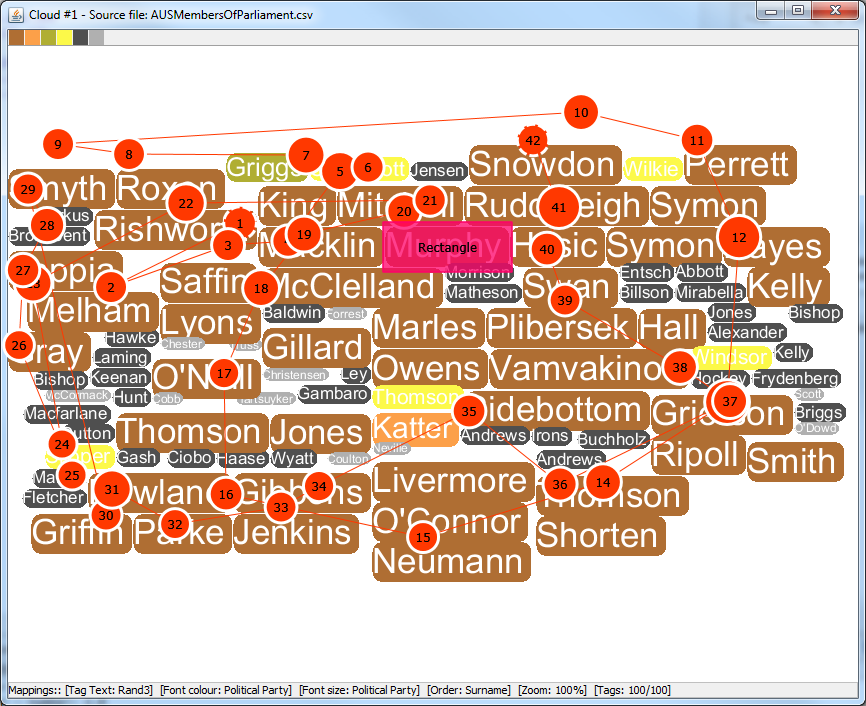
\includegraphics[scale=0.25]{t1chaoticsearch1.png}
  \caption{Repetition one with dual mapping}
\end{subfigure}%
\begin{subfigure}{.5\textwidth}
  \centering
  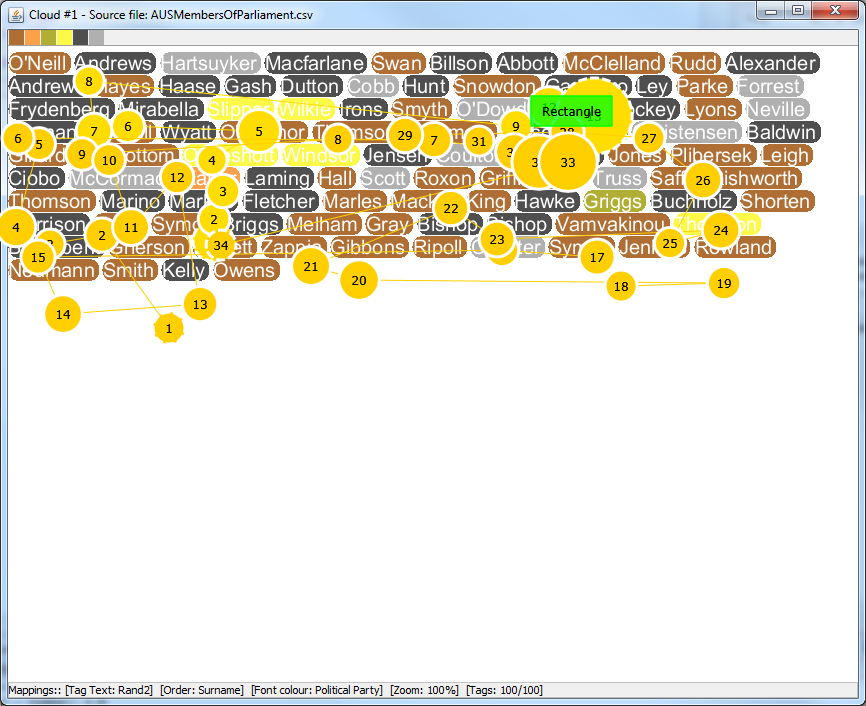
\includegraphics[scale=0.25]{t1chaoticsearch2.png}
  \caption{Repetition one with colour mapping}
\end{subfigure}
\begin{subfigure}{.5\textwidth}
  \centering
  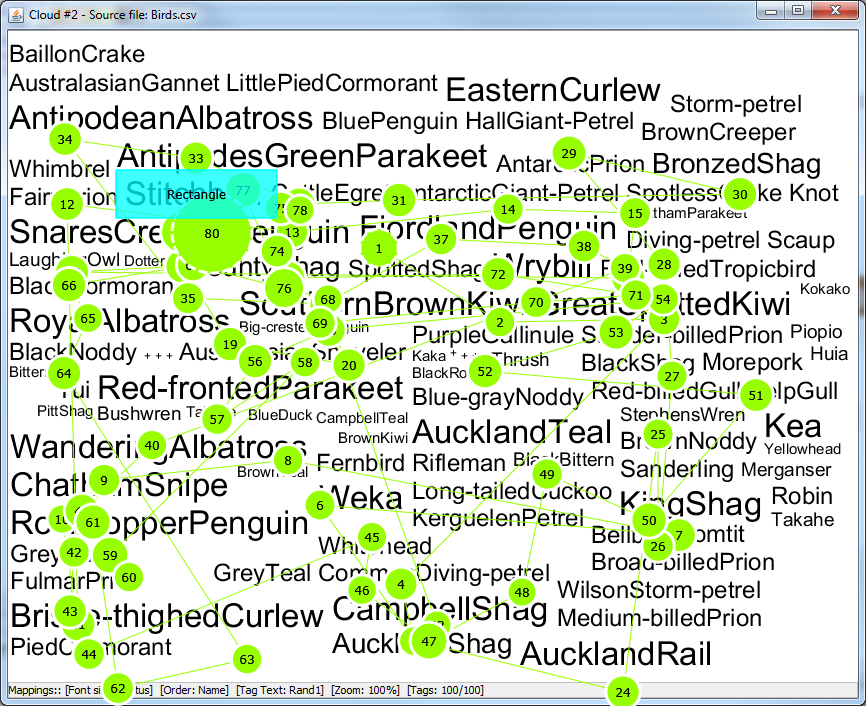
\includegraphics[scale=0.25]{t2chaoticsearch1.png}
  \caption{Repetition two with size mapping}
\end{subfigure}%
\begin{subfigure}{.5\textwidth}
  \centering
  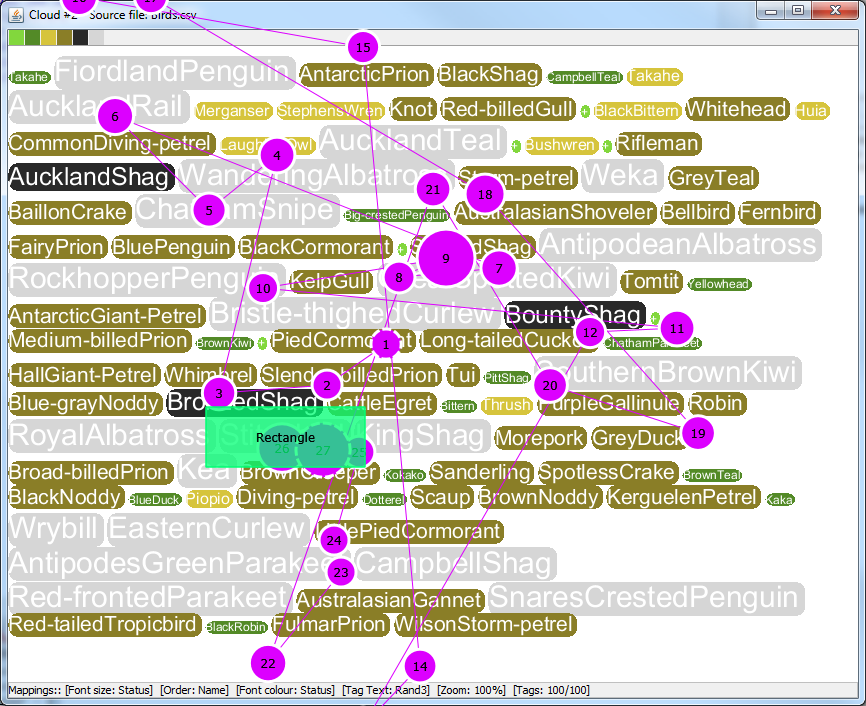
\includegraphics[scale=0.25]{t2chaoticsearch2.png}
  \caption{Repetition two with dual mapping}
\end{subfigure}
\caption{\textit{Visual searches with combinations of chaotic search, serial scanning and fixation clustering around tags with target mapping. Animated visualisations of these examples can be found at \url{http://www.cosc.canterbury.ac.nz/research/RG/svg/taggle/}}}
\label{fig:chaoticsearch}
\end{figure}

\subsection{Response time} \label{subsect:responsetime}

\begin{figure}[!htb]
	\centering
	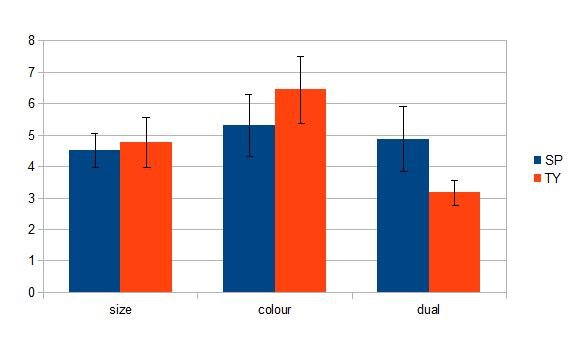
\includegraphics[scale=0.40]{exp2.jpg}
	\caption{\textit{Visual search response time in seconds}}
	\label{fig:exp2data}
\end{figure}

Figure~\vref{fig:exp2data} shows visual search response time across mappings (size, colour and dual) and layout type. While time differences in spiral layout don't appear to vary much between singular and dual mappings, there is a difference across the typewriter layout. Analysis of the tag cloud set-up in experiment one detailed in Chapter~\ref{chap:exp1} identified a possible bias in target location between the conditions. Therefore, data was also checked for bias in target location in experiment two.

Like experiment one, target location in experiment two was assigned randomly to a stimulus. We checked to see if randomly placed target positions had resulted in more unfavourable locations --- locations further away from the average first eye fixation --- for some experimental conditions. The average location of the first eye fixation across all conditions was calculated. This was again close to the stimulus midpoint, but further inside the upper left quartile --- see Figure~\vref{fig:exp2firstfix}.

\begin{figure}[!htb]
	\centering
	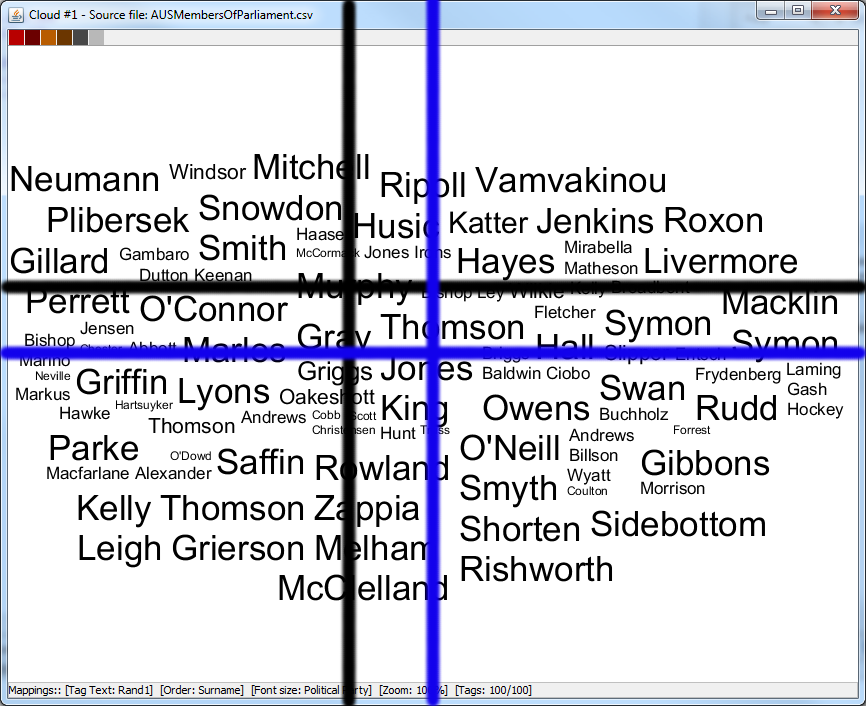
\includegraphics[scale=0.40]{averagefixation.png}
	\caption{\textit{Average location of first fixation (black) and stimulus midpoint (blue)}}
	\label{fig:exp2firstfix}
\end{figure}


The distance in pixels between the target tag and average location of first fixation for all stimuli was calculated (4 repetitions $\times$ 6 conditions = 24 visual stimuli). A pictorial representation of a subset of these can be seen in Figure~\vref{fig:fixationdata} where a) shows a favourably located target and b) shows a mildly unfavourably located target (representations of all 24 visual stimuli can be found in Appendix~\ref{appdx:eyegaze}). Average distance to first fixation (Figure~\vref{fig:fixations}) can be compared with response time results (Figure~\vref{fig:exp2data}). There is an average difference of 210 pixels to the first fixation point between spiral and typewriter layouts for the singular font size mapping. Despite this seemingly large difference, visual search average response times for singular font size mappings between spiral and typewriter layout are very similar ($t=4.51s$ and $t=4.77s$). It is unclear how much influence distance to average first fixation point has on search time.  

\begin{figure}[!htb]
\centering
\begin{subfigure}{.5\textwidth}
  \centering
  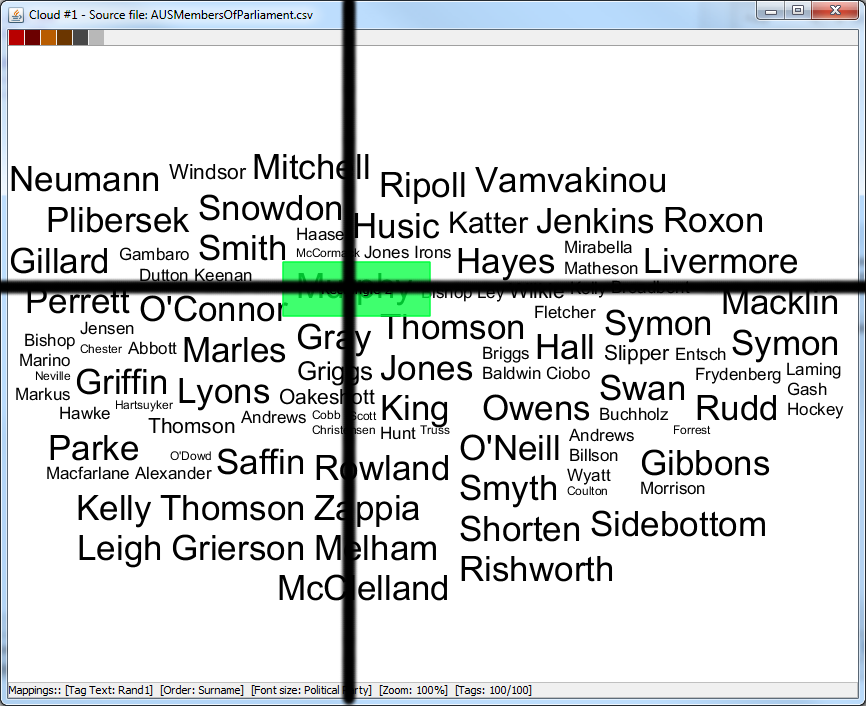
\includegraphics[scale=0.25]{M1Spiralfixation.png}
  \caption{}
\end{subfigure}%
\begin{subfigure}{.5\textwidth}
  \centering
  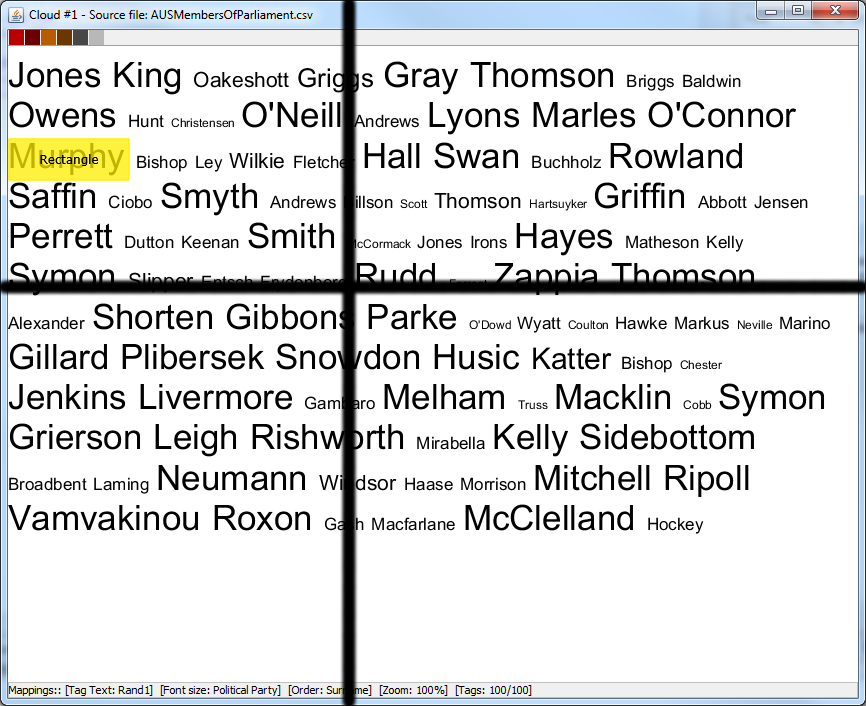
\includegraphics[scale=0.25]{M1Typewriterfixation.png}
  \caption{}
\end{subfigure}
\caption{\textit{Singular font size mapping, spiral and typewriter layouts}}
\label{fig:fixationdata}
\end{figure}

\begin{figure}[!htb]
	\centering
	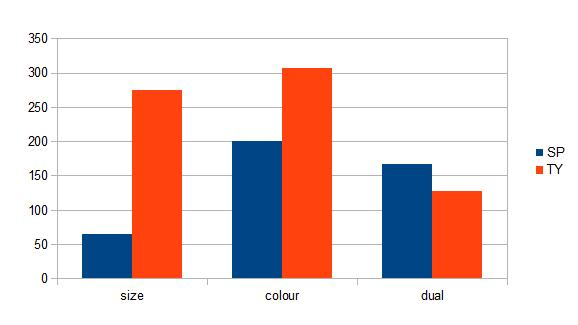
\includegraphics[scale=0.40]{fixations.jpg}
 	\caption{\textit{Average distance in pixels to first fixation}}
	\label{fig:fixations}
\end{figure}

For each condition in a repetition one of four categories for location was assigned; Favourable, Mildly Favourable, Mildly Unfavourable, Unfavourable. Assignation to location category was based on whether the distance was above/below median or 1st and 3rd quartile fixation values (see Table~\vref{table:locations}).

\begin{table*}
\centering
\caption{\textit{Target location favourableness per condition and repetition}}
\begin{tabular}{|p{3cm}|p{2.5cm}|p{2.5cm}|p{2.5cm}|p{2.5cm}|} \hline
\textbf{Stimulus}&\textbf{R1}&\textbf{R2}&\textbf{R3}&\textbf{R4}\\ \hline
size/spiral&Favourable&Favourable&Unfavourable&Favourable\\ \hline
size/typewriter&Mildly\par unfavourable&Mildly\par  unfavourable&Favourable&Unfavourable\\ \hline
colour/spiral&Mildly favourable&Unfavourable&Mildly favourable&Mildly favourable\\ \hline
colour/typewriter&Mildly\par  unfavourable&Mildly\par  unfavourable&Unfavourable&Unfavourable\\ \hline
dual/spiral&Favourable&Unfavourable&Mildly favourable&Mildly\par  unfavourable\\ \hline
dual/typewriter&Favourable&Favourable&Mildly favourable&Mildly favourable\\ \hline
\end{tabular}
\label{table:locations}
\end{table*}

Several outliers (seventeen) were calculated outside of three standard deviations from the condition mean. Only 29 percent of outliers were in groups with mildly unfavourable or unfavourable target locations, so outlier presence was not related to a poorer level of target location favourableness. The greatest factor correlated to the presence of outliers was repetition/dataset. Outliers were mostly contained to repetition one and repetition two (88 percent). The greatest number of outliers (11) were found in repetition two which had 21 data points in the target category, the next largest target category contained 16 data points and had no outliers. Outliers were spread fairly evenly across all eight conditions, and spread across all but one participant. Data distribution is positively skewed (see Figure~\vref{fig:exp2box}) --- skewness is characteristic of response times \citep[][]{luce86, zandt00, palmer11}). 

\begin{figure}[!htb]
\begin{subfigure}{\textwidth}
	\centering
	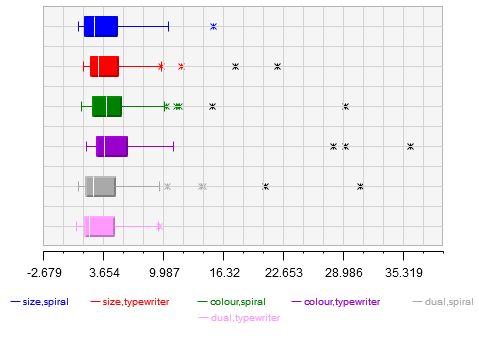
\includegraphics[scale=2.4]{boxplot.png}
\end{subfigure}
\begin{subfigure}{\textwidth}
  \centering
  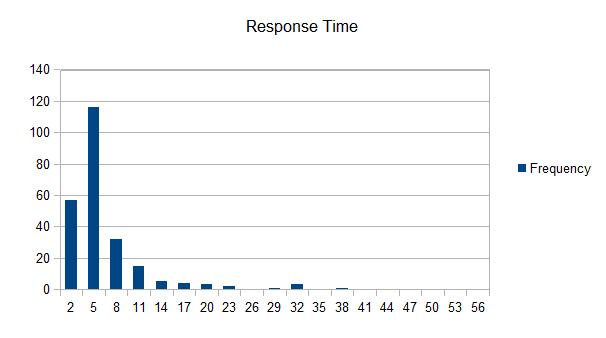
\includegraphics[scale=0.50]{distribution.jpg}
\end{subfigure}
\caption{\textit{Distribution of data}}
\label{fig:exp2box}
\end{figure}

Eye-gaze data for all outlying data points was also analysed.  Analysis of eye-gaze data concluded participants used primarily the mapping visual feature to aid their search for the target tag (\S\ref{subsect:eyegaze2}). However, when presented with a larger number of coloured targets such as in trial repetition one, participants appeared to resort to using a random search method or serial scanning to locate the target. 

The underlying dataset used in repetition two (containing the most outliers) had a target category with only 21 tags. Analysis of the dataset revealed a longer than average character length (11.46 characters compared to a range of 6.55\textendash7.69 characters for the other three datasets). Total characters in the dataset numbered 1146 compared to 722, 769 and 655 for the other datasets. The greater number of characters in the underlying dataset meant the tag cloud took up more space proportionally on the canvas than tag clouds from other repetitions. With the larger tag cloud filling up the canvas, participants appeared to be more likely to switch between search methods. 

Figure~\vref{fig:rep2} shows the eye-gaze data for two response time outlying values within repetition two. In this case participants applied a feature search with fixations clustered around tags with a large font size, but it appears that the larger tag cloud size resulted in making the search take longer than we might have expected (despite the target tag being in a potentially favourable location close to the average first fixation point). 

\begin{figure}[!htb]
\begin{subfigure}{.5\textwidth}
	\centering
	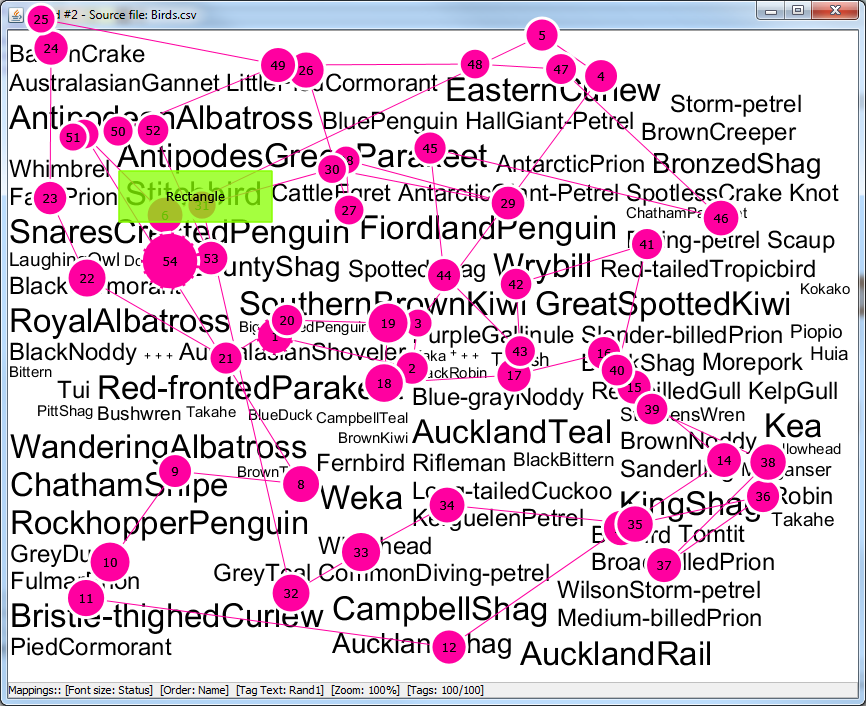
\includegraphics[scale=0.25]{t2sizespiralp3.png}
  	\caption{Participant three}
\end{subfigure}
\begin{subfigure}{.5\textwidth}
 	 \centering
 	 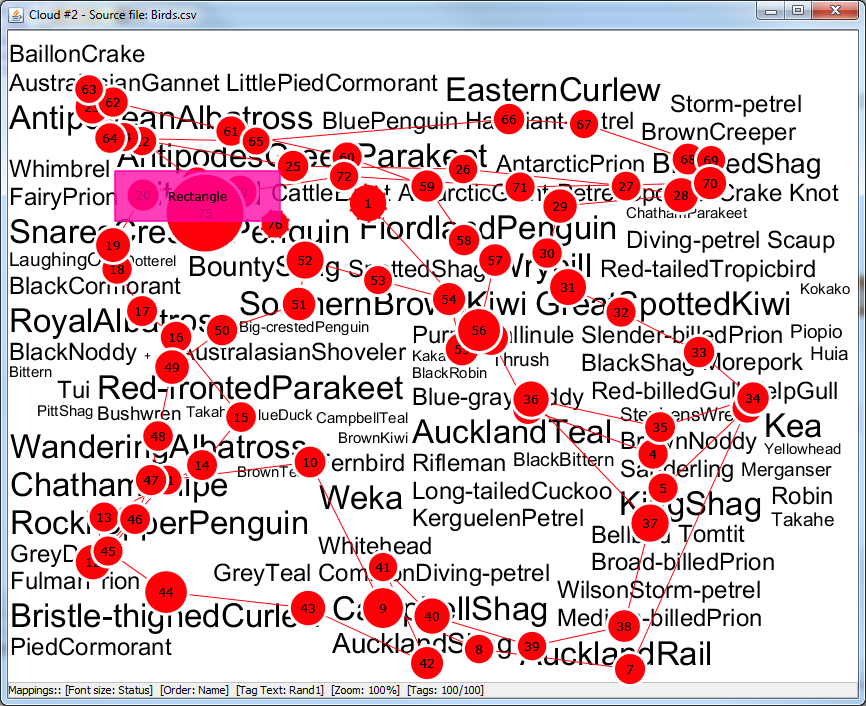
\includegraphics[scale=0.25]{t2sizespiralp6.png}
 	 \caption{Participant six}
\end{subfigure}
\caption{\textit{Gaze data for repetition two: size mapping, with spiral layout, response times are outlying values}}
\label{fig:rep2}
\end{figure}

Analysis of the response time data revealed the presence of several outliers and strongly positively skewed data. Careful examination of eye-tracking data showed outliers were due to a variance in either category size, or average tag length which increased the complexity of the task for the participant, rather than experiment procedure or participant error. 

\subsection{Significance testing}

A two-way ANOVA with repeated measures on the response times data showed a significant main effect for mapping ($F_{2,78}=7.93$, $p<0.000733$). Bonferroni-corrected pairwise comparisons showed the dual mapping of colour and size produced significantly faster visual search response times than singular size mapping ($t(39)=2.66$, $p<0.0113$) and singular colour mapping ($t(39)=3.93$, $p<0.0003$). This effect was achieved only when using the typewriter layout. Differences in search response time for mappings were not statistically significant in spiral layout, nor were the differences between singular size or colour mappings for either layout. All statistical testing was performed applying a logarithm transform so ANOVA data normality assumptions could be met. See Figure~\ref{fig:exp2log} for normalised response times for typewriter and spiral layout data.

\begin{figure}[h!]
	\centering
	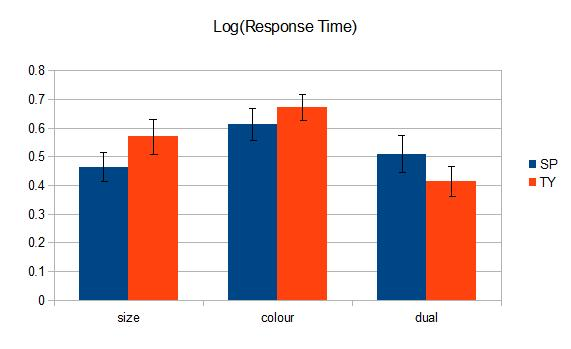
\includegraphics[scale=0.40]{exp2log.jpg}
	\caption{\textit{Normalised visual search response time}}
	\label{fig:exp2log}
\end{figure}

\section{Threats to validity}\label{sect:threatsexp2}

As in experiment one, there is the possibility that usage of genuine categorical datasets introduced bias by increasing the tag size of some tags through number of characters (this has been shown to have an effect on user perception of tag importance \citep{bateman08}). However, users were not identifying tags of subjective importance but searching for a specifically named tag. One dataset used (in trial repetition two) contained tags which had a larger average character length than datasets used in other repetitions. In experiment two, this resulted in that repetition containing a number of outliers with significantly longer response times to target selection. This dataset was used across all conditions so this shouldn't affect the comparison of the outcomes between conditions.

Some of the experiment conditions have (averaged across across all stimuli shown) an overall potentially more favourable target location than other conditions, although it should be noted it is not clear exactly what functional relationship there is between the average first fixation point and location of the target. This does not appear to have resulted in a clear pattern in the response times or impacted the conditions where outliers have appeared --- in fact, more outliers appeared in groups with favourable or mildly favourable target locations. 

\section{Summary and discussion}\label{sect:exp2summary}

Analysis of the visual search response time data revealed a difference between singular and dual mappings for typewriter layout. As with experiment one, a number of outlying data points were noted across the conditions. In experiment one the outlying data values were confined mostly to two repetitions, and were related to a large target category size (for one dataset, and the other dataset became an accidentally large target category size due to inappropriate colour palette choices).

In experiment two there were also two repetitions which contained most of the outlying data values -- one with a dataset with a large target category size, and one with a dataset with a long average tag length. It seems the long average tag length of this particular dataset was not a problem in experiment one when the target category size was very small (nine tags) but in experiment two, it suddenly became a problem when the category size was increased to 21. The extra number of characters in that particular dataset created a larger tag cloud filling up the canvas, and seemed to make it harder for people to find one individual tag (when they were searching for it within a larger target group of tags).

The dataset was used across all conditions (as was the large target category size dataset), but has caused some variability in the data, and probably contributed to the overall significant positive skew found in the data distribution. Therefore, like experiment one, all statistical testing was completed using a logarithm transform so data would conform to statistical testing requirements of normality.

\textbf{H1:} \textit{Mapping a data field to both tag font size and colour leads to faster visual search times than mapping a data field to either tag font size or colour separately, when the tag cloud was displayed in a typewriter layout.} Differences in search response time for mappings were not statistically significant in spiral layout, nor were the differences between singular size or colour mappings for either layout. As in experiment one, results were different for both layouts, and the reasons for this remain unclear. Further close analysis of the eye-tracking data could be performed in the future to explore this further.

Supporting the analysis of eye-tracking data in experiment one, the eye-gaze data for experiment two also indicates the introduction of a visual property hint in tag searches can alter the search strategy from serial scanning or chaotic search methods, to the eye scan path focusing on tags with the target mapping. 

\section{Conclusion and future work}\label{sect:exp2conclusions}

Our results indicate dual mappings of font size and colour as a data variable field can produce faster visual search response times than font size or colour alone. We think provision of multiple data mapping options to tag cloud visual properties in the Taggle interface highlights and reinforces the data mappings: this may help users identify data correlations and explore the data more effectively.

As with experiment one (Chapter~\ref{chap:exp1}), experiment two produced different results between the spiral and typewriter layouts, and future experimentation may help discover reasons behind this.

Varying target category size and average tag length over repetitions produced some abnormally long response times (outliers) for categories with greater sizes/tag lengths. Supporting our work from experiment one, eye-tracking data analysis showed when elements such as target category size or tag length increase the complexity of the task, participants tend to employ combination search methods switching between visual feature search, serial scanning and chaotic search. Future experiments may focus on the relationship between search methods and task complexity. 


% ------------------------------------------------------------------------


%%% Local Variables: 
%%% mode: latex
%%% TeX-master: "../thesis"
%%% End: 
